\documentclass[12pt]{article}
\usepackage{ucs}
\usepackage[utf8x]{inputenc}
\usepackage[T1]{fontenc}
\usepackage[english]{babel}
\usepackage[nottoc]{tocbibind}
\usepackage[left=2.5cm,right=2.5cm,top=2.5cm,bottom=2.5cm,]{geometry}
\usepackage{graphicx}
\usepackage{nameref}
\usepackage{hyperref}
\usepackage{sidecap}
\usepackage{wrapfig}
\usepackage[bottom,hang]{footmisc} 
\usepackage{acronym}
\usepackage{multirow}
\usepackage{color}
\usepackage{capt-of}
\usepackage{array,				%better tables
			tabularx,			%instead of tabular*             
			booktabs,			%tables for good publications
}
\usepackage{afterpage,hyperref} 
\usepackage{listings}
\lstset{
    basicstyle=\ttfamily\footnotesize,
    numbers=left,
    xleftmargin=15pt,
}


%--------------------------MAKETITLE-------------------------------%
\title{Technologies and Design of Graphical \\ 
and Virtual User Interfaces: \\
Application Areas of Augmented and Virtual Reality}
\date{\today}
\author{Mehmed Mustafa \\
		MatrNr: 21914377 \\
		Supervisor: Patrick Harms} 

\begin{document}
%--------------------------BEGINNING-------------------------------%
\pagenumbering{roman} 
\maketitle
\thispagestyle{empty}
\newpage
\tableofcontents
\newpage

%-----------------------SECTION START------------------------
\pagenumbering{arabic}

\section{Introduction} \label{sec:Introduction}
Technology has always been a very important aspect for us, humans, since the dawn of humankind. Two technologies, named \ac{VR} and \ac{AR}, are expected to be part of our daily life in the near future. Although they can be considered as a single technology, there are differences, which should be clarified, so it is easier to understand how they could be applied in different application areas. One difference is that \ac{VR} creates completely new virtual environments (worlds), while \ac{AR} augments (adds to) real-life environments with the aid of digital objects. In other words, users experiencing \ac{VR} cannot see the real-world around, since they are fully immersed in the action. On the other hand, with \ac{AR}, users are able to see the real-world around and are, in fact, only partially immersed in the action. In order to experience \ac{VR}, a special equipment (\ac{VR} headset) is needed. There are various options available on the market, from high-end to low-end, such as HTC Vive, Oculus Rift, Google Daydream or Google Cardboard. For experiencing \ac{AR}, however, a special equipment is not a must. Most of the current generation smartphones support \ac{AR}.  But it should be kept in mind that current generation smartphones were not specifically designed for \ac{AR} experiences, and thus using an \ac{AR} headset will provide more advanced experience. Maybe in the future smartphones will be better tuned for such experiences and able to run \ac{AR} applications more smoothly. Estimation of the \ac{VR} and \ac{AR} market size is not an easy task. According to Statista~\cite{statista}, a German online portal for statistics, predicted market size for \ac{VR} and \ac{AR} software in 2025 was estimated to reach \$35B. The interesting thing about this statistic is that it is from 2016 and already outdated because according to the same source the market size for 2019 is already around \$35B and their new market size prediction for 2023 is \$160B. It could be thereby expected that these technologies have future and it is of importance to know their application areas. But before going to application areas section, it is a good idea to have a look where do \ac{VR} and \ac{AR} take place at \ac{GHC}, so it is possible to estimate when these technologies could be massively used. \ac{GHC} is a good model for understanding the spread of new technologies. It states that as a technology first appears people get excited and their expectations get inflated by big tech companies (Peak of Inflated Expectations). But as soon as the first products come out and the provided experience does not match the inflated expectations, consumers give up very quickly and lose hope in that technology (Trough of Disillusionment). Of course, if a technology has some potential, companies will keep investing in and developing it until they fix the major early problems (Slope of Enlightenment). Eventually, people will then start seeing the benefits again and companies will make a lot of profit from mass production once the technology gets mature (Plateau of Productivity).~\cite{gartnerPrediction} Check Figure~\ref{fig:gartnerCycle}. In 2017, according to \ac{GHC}, it was expected that in the next 2 to 5 years \ac{VR} and 5 to 10 years \ac{AR} will reach complete market maturity. However, in 2018 \ac{VR} and in 2019 \ac{AR} were excluded from the cycle claiming that they reached the Plateau of Productivity. For some technology experts~\cite{gartnerCounter} this behavior is questionable, because \ac{VR} and \ac{AR} technologies are still being tested and they are by no means mature. The maturity, according to them, is reached once a technology is already used in companies in the form of various applications. \ac{VR} and \ac{AR} may be ready for the market, but for maturity state some more years are needed, since there are still problems which have to be solved. Section 2 overviews different application areas of \ac{VR} and \ac{AR}, Section 3 discusses current issues with them and Section 4 concludes. 

\begin{figure} [ht]
    \centering
    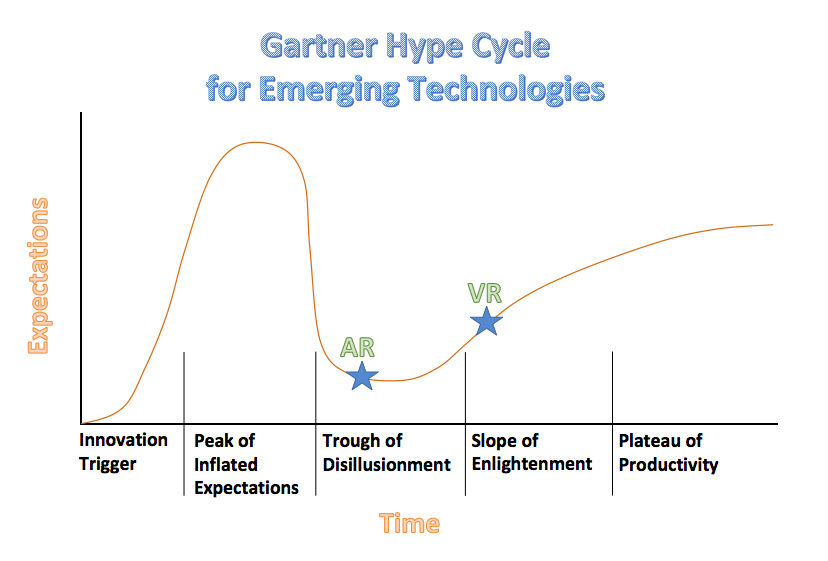
\includegraphics[width=0.80\textwidth]{../images/Gartner.png}
    \caption{\ac{VR} and \ac{AR} on the \ac{GHC} graph, 2017~\cite{gartnerPrediction}.}
    \label{fig:gartnerCycle}
\end{figure}

%---APPLICATION AREAS---

\section{Application areas of Virtual and Augmented Reality} \label{sec:Application areas of Virtual and Augmented Reality}
This section explores some of the ways \ac{AR} and \ac{VR} have been used in various industries or how they could be used in the future. Instead of concentrating only on the specific \ac{AR} and \ac{VR} applications being discussed, try to think critically about other possible usages of these technologies that have not yet been discussed. Although it is wrong to consider that \ac{AR} and \ac{VR} technologies are only used for entertainment, mainly for games, a lot of users make this kind of wrong conclusions. This is no surprise since mass of them were introduced to \ac{VR} and \ac{AR} with applications created for entertainment purposes. Indeed, these technologies can provide engaging entertainment experiences, but the application areas are far beyond the entertainment sector. \ac{AR} and \ac{VR} will shine in their true potential only when the mass user understands how these technologies may be used in different sectors.

\subsection{Health-care} \label{sec:Health-care}
Ian Pilkington, the director of \ac{AR}/\ac{VR} Solutions at Arm Holdings, mentions in his blog~\cite{healthCare} some of the ways \ac{AR} and \ac{VR} are revolutionizing the health-care sector. Both technologies are having positive impacts on the physical and mental health of patients. In addition, they can be also helpful for understanding of various health conditions and diseases, and thus provide better understanding for professionals from different spheres. Also in comparison to other technologies, \ac{AR} and \ac{VR} smart devices are more accessible and cheaper.

\subsubsection{Pain management} \label{sec:Pain management}
\ac{VR} can be used to effectively reduce pain feeling by affecting the brain's neural pathways by putting patients in different environments which provide experiences close to real-life ones, and thus helping them to forget about the pain they are suffering from. According to the company~\cite{healthCare} which developed this \ac{VR} application, using of it led to a 52 per cent reduction in pain among patients.

\subsubsection{Phobia treatment} \label{sec:Phobia treatment}
Researchers from The Polytechnic University of Valencia came with an idea of \ac{AR} application~\cite{phobia} which could be used for treating several psychological problems, such as phobias to insects and small animals. They believe that the \ac{AR} technology gives greater feeling of presence than the \ac{VR} one because during a treatment users are seeing their own body parts rather than virtually simulated ones. The participants of the study were asked to rate their anxiety during the exposure and after the treatment. All of them had on average 70 per cent lower levels of anxiety after the treatment. However, the number of test subjects was only 9. This small sample size may not be enough for a conclusion about the effectiveness of the application. Figure~\ref{fig:phobia} shows an example view of spiders approaching a participant.

\begin{figure} [ht]
    \centering
    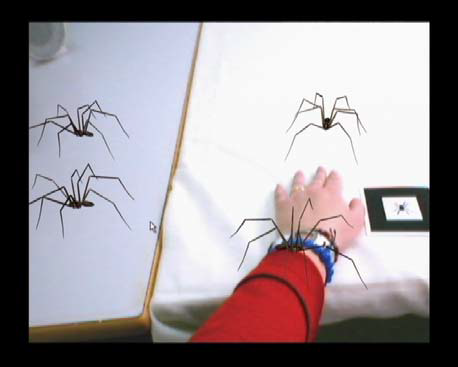
\includegraphics[width=0.45\textwidth]{../images/phobia.png}
    \caption{Spiders approaching a participant.~\cite{phobia}.}
    \label{fig:phobia}
\end{figure}

\subsubsection{Identifying the early signs of schizophrenia} \label{sec:Identifying the early signs of schizophrenia}
"Schizophrenia is a psychiatric disorder that affects around one in 100 people worldwide with common symptoms such as delusions and auditory hallucinations, or hearing voices. At present, there is no single test for schizophrenia and the condition is usually diagnosed after assessment by specialists in mental health."~\cite{schizophrenia} A group of researches~\cite{schizophrenia} and experts from the University of Exeter have developed a 'mirror game' in order to try to identify the early stages of schizophrenia. The players of the game were placed in front of a large screen and were instructed to mirror the movements they were seeing. They were also instructed to perform specific movements on their own. The movements which had to be performed had been selected according to well-documented characteristics related to the mental disorder. In comparison to other traditional neuroimaging methods, which are more expensive, the results from the 'mirror game' were more accurate. According to the researches the 'mirror game' test can not only give quick and accurate diagnosis, but also to validate the effectiveness of ongoing treatments.

\subsection{Education} \label{sec:Education}
One of the biggest difficulties teachers may face is to make their students excited about learning. \ac{AR} and \ac{VR} technologies could be useful in education sector because they can manage to increase the interest rate of students and make them more engaged to the learning material. More connected to the material they are, it is more likely that they will retain the presented information. Moreover, students whose needs may not be satisfied in a passive-learning environment, could get a better understanding of the learning material with the aid of \ac{AR} and \ac{VR} technologies. Google Expeditions, a collection of \ac{AR} and \ac{VR} applications, is a really good example of the high potential of these technologies in the education sector. With Google Expeditions \ac{AR}~\cite{googleExpeditionsVideo} students can augment their classrooms with different objects, such as volcanoes, tornadoes, asteroids etc., which may help them for better understanding of their physical characteristics. Especially, for anatomy classes being able to see the details of the organs of the human body makes learning a lot more easier. Google Expeditions \ac{VR}~\cite{googleExpeditionsVRList} offers various expeditions to different destinations of the world or time travel to historical places. Students have a lot of places to explore. 

\subsection{Military} \label{sec:Military}
Michael Morozov, the founder and CEO of a software development company which builds \ac{AR} and \ac{VR} applications, shares his experience about the usage of these technologies in the military sector~\cite{military}. According to him emerging technologies have always been firstly used in the military sector, so the training of soldiers and combat enhancements are at their full potential. Long before the mass user was aware of the existence of \ac{AR} technology, it was already used in the military for real-time overlaying of all the crucial information onto the fighter-jet pilot's visor, so it is not needed to look down on panels, which increased the concentration rates of the pilots. With the advancement of graphical and data processing, usages of \ac{AR} has increased even more. Further use of \ac{AR} in the military is a system called "Tactical Augmented Reality", which is similar to night-vision goggles and is mounted the same way on the helmet of soldiers. The system can operate both during day and night, and provide functionality of \ac{GPS}, by showing the exact locations of ally and enemy forces. Moreover, soldiers are able to identify the targets, they are aiming at, more precisely and see the distance to them. It is also possible to divide the screen view in two parts, one part - showing the position where the gun is pointing, the other part - showing the view of frontal camera, which allows soldiers to see over a wall or around a corner without any risks of being shot. Best of all, sharing information among the squad members is possible because the system has its own wireless network.

\subsection{Engineering and Industry}\label{sec:Engineering and Industry}
\ac{AR} and \ac{VR} technologies could be used in variety of industrial enterprises and engineering fields. Enrico Kabbe, owner of ARTS, a company which develops \ac{AR} and \ac{VR} applications for the industry sector, describes some of the industry usages in his blog~\cite{industry}. With the usage of AR technology, for example, designers and engineers are able to design different prototypes and make decisions about their physical characteristics before the actual prototypes are built. Workers on the other side, are able to optimize assembly processes and do manual manufacturing with less mistakes. Moreover, production processes can be covered visually, and thus reducing the number of faults and errors. Figure~\ref{fig:automotive} shows an example AR application which gives instructions to a mechanic. With the help of this application new employees may be trained faster than with a guidance of a supervisor. Moreover, the application can greatly reduce the number of mistakes made from employees, especially new ones.

\begin{figure} [ht]
    \centering
    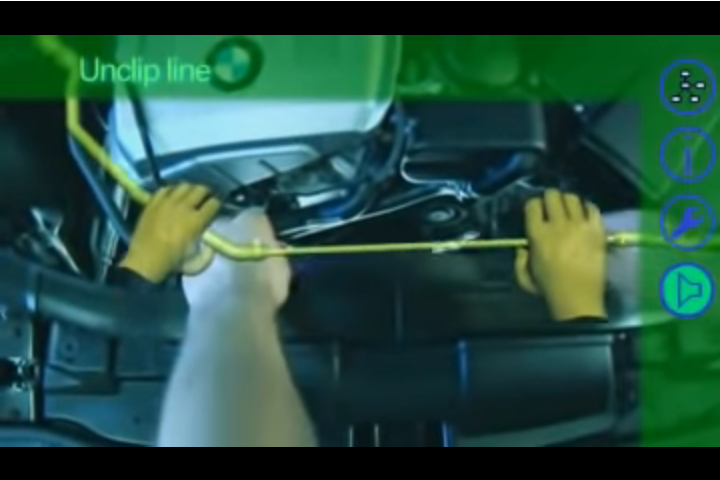
\includegraphics[width=0.65\textwidth]{../images/BMW.png}
    \caption{AR guides the mechanics in Automotive industry~\cite{industry}.}
    \label{fig:automotive}
\end{figure}

\subsection{Food Sector} \label{sec:Food Sector}
Food industry is yet another sector, in which the \ac{AR} and \ac{VR} technologies could dominate. Example applications related to this sector are discussed by Bhagat~\cite{food}. Customers are an important aspect of each industry because they decide the growth rate of that industry. Satisfaction and engagement of customers to a given set of products is crucial for achieving high revenue. One way of keeping customers engaged and interested might be by using a \ac{VR} application which shows them how their dish is prepared. Another way might be by using an \ac{AR} application which overlays additional information on top of a menu. For example, showing the ingredients of each dish on the menu. Rollo et al.~\cite{servAR} were able to accurately estimate food portion size by using an \ac{AR} application they have developed. This application, named "servAR", may come in quite handy for people wanting to easily track their portions on daily basis. Moreover, it could be used in environments such as restaurants where the size of portions should be same.

\subsection{Real Estate} \label{sec:Real Estate}
Gleb B. examines in his blog~\cite{realEstate} how the real estate sector is innovated by using various \ac{VR} applications. For decades the process of buying or selling a property remained same. An agent gets all specifications about a desired property from a client and makes suggestions to the client with various properties currently available on sale, which match the requirements of the client. Then negotiations between the agent and the client take place. The final step is to visit the chosen apartments and/or houses. Buying a property by dint of a real estate agent, may be an inconvenient and time-consuming process. However, \ac{VR} applications can significantly shine in this sector and change the way it is working. Instead of visiting a lot of properties and wasting time, clients could just put their \ac{VR} headsets and visit the places in a virtual environment. Afterwards they could decide which ones they would like to see in real-life. Real estate agents, on the other hand, could add furniture on a virtual level, which is not present in the real-life apartment, so it looks more cozy for the buyers. According to a research~\cite{realEstateResearch} of \ac{NAR}, furnished properties are more easily associated as a 'future home' by a buyer. Moreover, agents are able to sell furnished properties for a higher value than their authentic one.

\begin{figure} [ht]
    \centering
    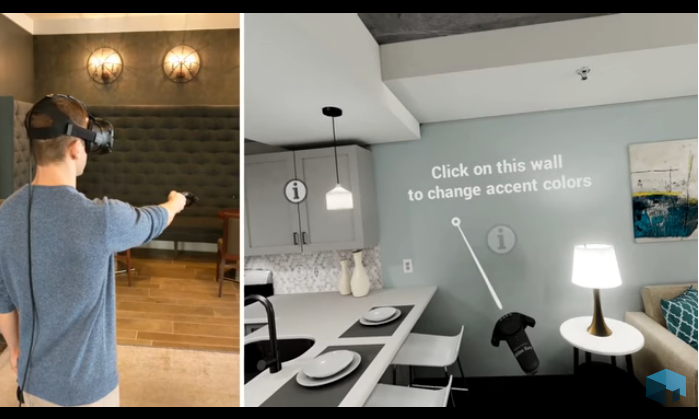
\includegraphics[width=0.65\textwidth]{../images/realEstate.png}
    \caption{Buyer observing an apartment using \ac{VR}~\cite{realEstate}.}
    \label{fig:realEstate}
\end{figure}

\subsection{Entertainment} \label{sec:Entertainment}
Entertainment sector, as mentioned before, for the mass user, is the most obvious sector, in which \ac{AR} and \ac{VR} can be used. For example \ac{VR} can be used in theaters for fully immersing the audience into the action. Another use case may be for music concerts. Users can put their \ac{VR} headsets at home and enjoy a concert from their home. Possible usage for \ac{AR} might be in galleries and museums. In Galleries people could get additional information about an artist or other information related to pictures. In museums, for example, users could see the living version of prehistorical creatures, like dinosaurs, as a hologram.


%---CURRENT ISSUES
\section{Current issues with Virtual and Augmented Reality}\label{sec:Current issues with Virtual and Augmented Reality}

Paul Mealy has briefly described in his book~\cite{dummies} the most relevant issues in front of \ac{VR} and \ac{AR} on their path towards the mass consumption state. The following subsections are discussing these issues covered inside the book. 

%---VR
\subsection{Current issues with Virtual Reality}\label{sec:Current issues with Virtual Reality}
In the recent years the availability of \ac{VR} devices has increased and their price decreased, but there are still some technical issues which should be overcome in order to make \ac{VR} reach its mature state. However, since companies are getting more and more interested in \ac{VR}, and thus investments in the field are growing, it is expected that the process of solving the current issues will be accelerated.

\subsubsection{Simulator sickness} \label{sec:Simulator sickness}
Early mass consumer \ac{VR} devices were not successful. A lot of users, after usage of headsets for some time, were complaining of headaches, nausea, dizziness, and disorientation. These symptoms are caused from the brain of the user due to inconsistency in signals between what the eyes see and what the inner ear's vestibular sense of motion senses. This phenomenon is known as motion sickness. However, there are also cases in which a motion sickness could occur even when there is no motion involved while using a \ac{VR} headset. Nowadays, at the time of writing this report, headset manufacturers are still trying to resolve this issue. Since a motion sickness occurs because of signal inconsistencies, one logical solution would be to make these signals consistent by decreasing the response time of VR headsets to user's real-world actions. In the perfect case there should be no latency at all, in order to give the user the real-world experience. Theoretically, the motion sickness effect should be resolved as more powerful devices are introduced, because they will be able to handle all kind of interactions smoothly, thus reducing the latency to minimum. One study~\cite{nasumVirtualis}, in order to confront motion sickness, introduced "virtual nose", which acts like a stabilizer. They reported that users were able to spent 94.2 seconds more time in the Tuscany villa simulator, which according to them is a huge improvement.

\subsubsection{Movement} \label{sec:Movement}
Another issue with \ac{VR} is the movement through the virtual environment. Even with the most capable headsets available on the market, user actions could be tracked at most within a room. Moving over large distances will remain a main problem, because of several reasons. Firstly, trying to simulate movement without involving physical movement of a user could provoke simulator sickness, even when there is no response delay from headset's side. Secondly, laziness may be another factor. Users may not want to traverse large distances by physical walking. Lastly, disabled users, which are not able to cover distances on foot, should also be considered. Solving the movement issue would not be an easy task for developers.

\subsubsection{The screen-door effect} \label{sec:The screen-door effect}
The screen-door effect occurs when the resolution supported from a \ac{VR} headset is low and insufficient. Users having such headsets may be able to notice black lines in-between the screen pixels. This effect was first introduced with televisions, but has been solved with high enough resolutions. The same approach may be a feasible solution for \ac{VR} headsets, in order to diminish the screen-door effect. However, higher resolution screens will require more processing power, which may not be an option for the current generation of \ac{VR} headsets. Figure~\ref{fig:screen_door} shows an example of the screen-door effect.

\begin{figure} [ht]
    \centering
    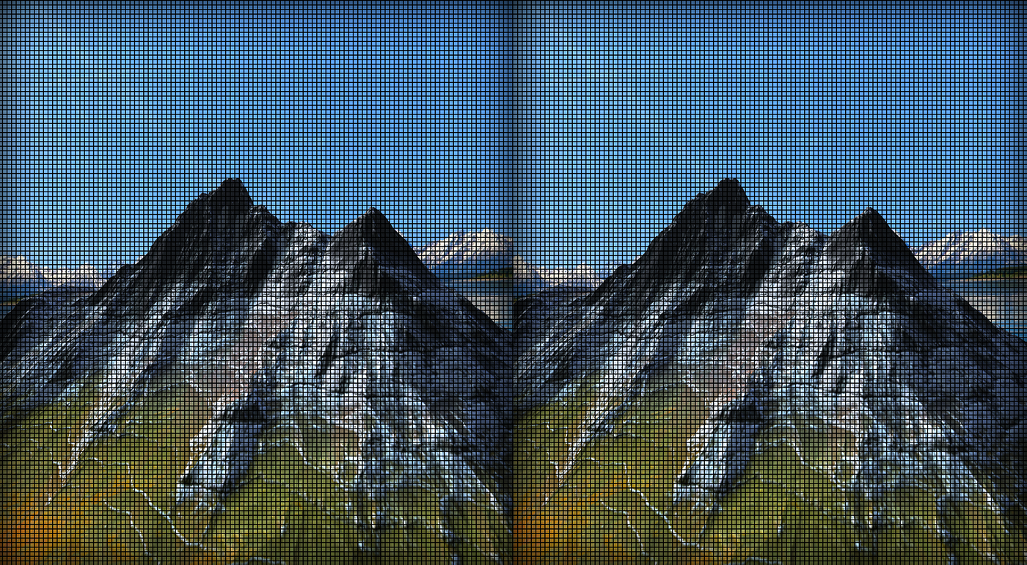
\includegraphics[width=0.65\textwidth]{../images/screen-door.png}
    \caption{Screen-door effect~\cite{dummies}.}
    \label{fig:screen_door}
\end{figure}

\subsubsection{Health risks} \label{sec:Health risks}
The time spent in a \ac{VR} environment is relatively short compared to the time spent by playing video games. Thus, long-term health effects are still unknown. Researchers still have to conduct researches to find out the impact of \ac{VR} headsets on eyesight and the brain in case of a long-term usage. The Health and Safety guidelines for some \ac{VR} headsets, for example Oculus Rift, warn that blackouts, seizures and severe dizziness might be experienced.

%---AR
\subsection{Current issues with Augmented Reality}\label{sec:Current issues with Augmented Reality}
According to prediction of \ac{GHC}~\cite{gartnerPrediction}, a global technology research firm, mass adoption of \ac{AR} 
will occur some years after \ac{VR} adoption. This is expected according to Paul and stated in his book~\cite{dummies} as follows: "\ac{AR} shares almost all the same issues \ac{VR} experiences but has the additional issues to solve of computer vision for detecting real-world objects, unique display form factors on transparent displays (if not using a video camera as pass-through), digital object placement, locking digital holograms in place within the real-world, and much more."

\subsubsection{First impression}\label{sec:First impression}
At first glance, the integration of \ac{AR} features to smart-phones may be seen as an advantage, because millions of users are able to experience \ac{AR} without the need of buying some special expensive equipment. However, this first experience will be very poor, since the standard smartphones were not designed optimally for \ac{AR}, and thus users will get wrong impression about the possibilities of \ac{AR} technology and dismiss an advanced experience which could be provided by a special \ac{AR} equipment.

\subsubsection{Cost and Availability} \label{sec:Cost and Availability}
In addition to the first impression problem, there is also an availability problem. Most of the available \ac{AR} headsets on the market, at the time of writing this report, are mostly targeting either developers or enterprise, since the prices are high and unbearable for regular users. There are available some cheap options for \ac{VR} headsets, but this is not the case for \ac{AR} ones. This may be an additional reason for the slowed down process of mass adoption of the \ac{AR} technology.

\begin{figure} [ht]
    \centering
    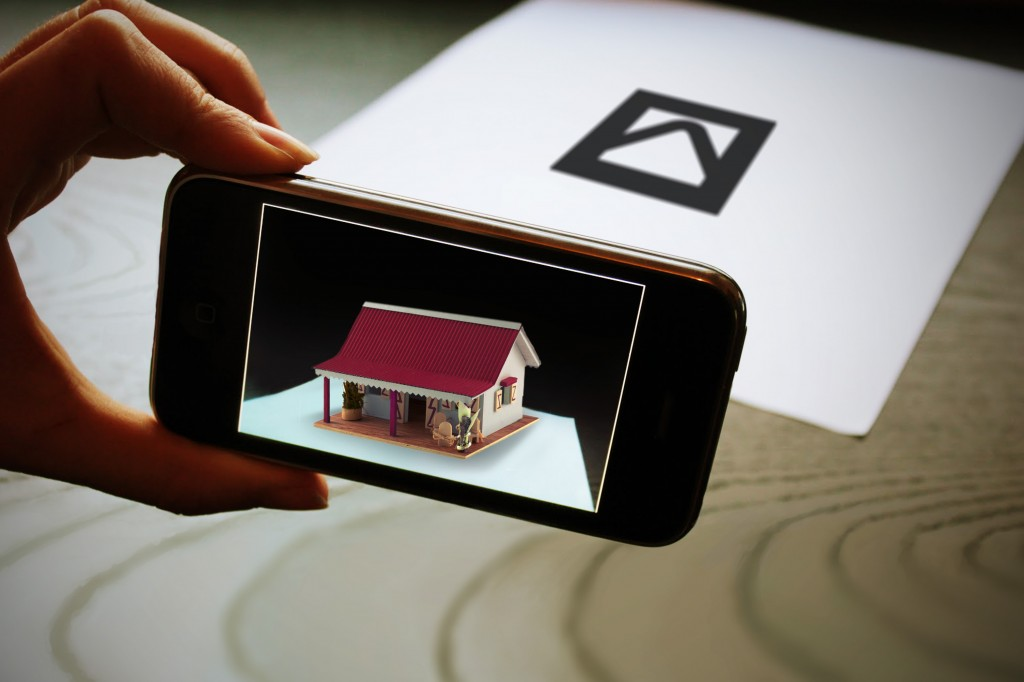
\includegraphics[width=0.50\textwidth]{../images/ar-marker.jpg}
    \caption{Marker-based AR~\cite{arMarker}.}
    \label{fig:ar_marker}
\end{figure}

\subsubsection{Tracking} \label{sec:Tracking}
Computer vision plays an important role when it comes to \ac{AR} technology. "Understanding" the surrounding real-life environment is a key for a device, in order to activate main features of \ac{AR}, such as placing digital objects in real-world's three-dimensional space. The brain of a human can easily distinguish among different objects, such as a table, a chair or a window, in a scene, but this is not an easy task for a computer because the only thing it will see is a number of pixels with no meaning. Computer vision describes how a computer can not only understanding what a collection of pixels may represent, but also to identify the shape of an object and its depth in a three-dimensional space. One of the biggest challenges that \ac{AR} still faces today, is the tracking. Tracking of the surrounding environment is the most important variable in the \ac{AR} technology, in order to successfully match the place of digital objects on top of the real environment. Placing objects by using specifically designed markers is easier. They are showing the exact location, where an object should appear, and thus the only thing a device should try to recognize is that specific marker. Check Figure~\ref{fig:ar_marker}. However, the goal of most \ac{AR} applications is a tracking without using any markers. Most of the available \ac{AR} devices, even being able to meet the high requirements to do marker-less tracking, they are still suffering from tracking delays. For example, shifting of digital objects, placed on top of a surrounding real-life environment, may occur in case the device is moved quickly around. Nowadays, the tracking issue is still present.

\subsubsection{Perceived usefulness}\label{sec:Perceived usefulness}
Another issue of \ac{AR} arises from the fact that many people do not understand what they would use it for, although they are interested in it. The benefits of \ac{VR} are more obvious, because virtual worlds were popularized by books, movies and popular media in general. On the other hand, \ac{AR}, was not exposed that much to the public eyes and it is just gaining its popularity. Although there are already some applications which show the usage of \ac{AR}, regular users are still not convinced to invest huge amount of money in \ac{AR} equipment. This, on the other side, makes software developers to no want to invest their time in developing \ac{AR} apps, since the \ac{AR} hardware has not reached its mass adoption. Seems like the first developers which succeed to develop the must-have \ac{AR} applications will dominate the AR sector and will generate huge amount of income.

\subsubsection{Field of view} \label{sec:Field of view}
"\ac{FOV} refers to the space in which digital holograms can appear. For example, the \ac{FOV} for mobile \ac{AR} is the amount of view-able space on your device screen. The device screen acts as your window into the \ac{AR} world. Look away from this window into the digital, and you would only see the real-world, where no holograms exist."~\cite{dummies}
 
\begin{figure} [ht]
    \centering
    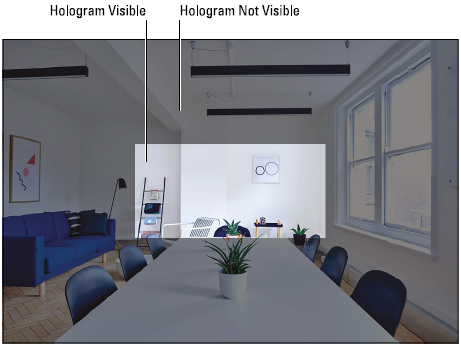
\includegraphics[width=0.65\textwidth]{../images/hologram-visibility.png}
    \caption{Hologram visibility~\cite{dummies}.}
    \label{fig:hologram_visibility}
\end{figure}

Figure~\ref{fig:hologram_visibility} shows an example view from an \ac{AR} headset. The digital objects added to the physical world would be visible only in "Hologram Visible" area. Everything else which appears in "Hologram Not Visible" area would be invisible. If a hologram appears between the two areas only the part which fits into "Hologram Visible" area will be visible. It can be clearly seen that larger \ac{FOV} has an advantage and can provide better immersion for the users. The human eye has a \ac{FOV} of approximately 200 degrees horizontally and 135 degrees vertically, but the \ac{AR} devices, currently, are able to provide at most 90-degree \ac{FOV} which is greatly limited. It will take some time till the \ac{FOV} of devices reaches the \ac{FOV} of the human eye.

\subsubsection{Visuals} \label{sec:Visuals}
High-resolution demands are problem for both of the current generations \ac{VR} and \ac{AR} headsets. There is an additional issue for \ac{AR} devices - poor occlusion. Occlusion means that physical objects may block digital ones, and thus causing them to half-stuck somewhere. If the occlusion was properly executed, digital objects would have been placed more accurately and realistically in a real-world environment. In other words, if the \ac{AR} devices were able to perfectly detect all objects in the physical world, they would have known exactly how to place digital objects and decide which objects should be in the background and which in the foreground. In order to maximize the immersion effect, occlusion should be solved.

%---CONCLUSION---

\section{Conclusion} \label{sec:Conclusion}
\ac{VR} and \ac{AR}, like other technologies, have both positive and negative sides. The positive sides were discussed in the application areas section. The negative sides should be also considered for a better view of the whole picture. Since \ac{VR} is fully immersive, it is likely to suffer from the same problems as the computer games suffer in general. Addiction will be the main problem. Users may start spending a lot of time inside a virtual world and start to forget their connection with the real one. Another possible issue may be that the users will get less sensitive in the real-world because of lack of consequences of their actions inside a virtual world. \ac{AR}, although not fully immersive, has its issues. What if digital objects added on top of the real-world become very realistic, so that after some time of using \ac{AR}, users are no longer capable to distinguish what is real and what enhanced ? Other concern is related to the ownership of a digital world. There are 2 questions which should be answered: "Should anyone has the possibility to display digital objects whenever and wherever they want ?" and "Could a digital content harm in some way the reputation of other people or institutions ?". Although there are negative sides of these technologies, their positive potential, as seen in application areas section, surpasses their negative sides and if users are conscious about the negative sides, they may be able to avoid them. Paul Mealy, in his book~\cite{dummies}, evaluates the future of \ac{AR} and \ac{VR} as follows: "\ac{VR} has the ability to reach across boundaries and borders. The Internet connected people like never before. \ac{VR} takes that power and adds in the ability to form a truly empathetic global social space. It has the capability to completely revolutionize how we learn and how we play, and perhaps most importantly how we connect with one another. \ac{AR} has the ability to enhance our everyday actions within the real-world. It has the potential to help people make smarter decisions via information availability. It can make the world around us interactive. It can facilitate creating new connections with others via shared experiences and change the ways we currently work. You name the industry, and within ten years, \ac{AR} may have massively transformed that industry as we know it." 


\newpage
%-------------------References---------------------------%
\section*{Abbreviations and Acronyms}
\addcontentsline{toc}{section}{Abbreviations and Acronyms}

\begin{acronym}[Bash]
	\acro{AR} {\textit{Augmented Reality}}
	\acro{FOV} {\textit{Field of view}}
	\acro{GHC} {\textit{Gartner Hype Cycle}}
	\acro{GPS} {\textit{Global Positioning System}}
	\acro{NAR} {\textit{National Association of Realtors}}
	\acro{VR} {\textit{Virtual Reality}}
\end{acronym}

%----------------List-of-Tables--------------------%
%Comment the following lines out if you dont have tables or figures
%\listoftables
\listoffigures
\bibliographystyle{plain}
\bibliography{lit}
\end{document}
